\thispagestyle{toancuabinone}
\pagestyle{toancuabi}
\everymath{\color{toancuabi}}
%\blfootnote{$^1$\color{toancuabi}Đại học Thăng Long.}
\graphicspath{{../toancuabi/pic/}}
\begingroup
\AddToShipoutPicture*{\put(0,616){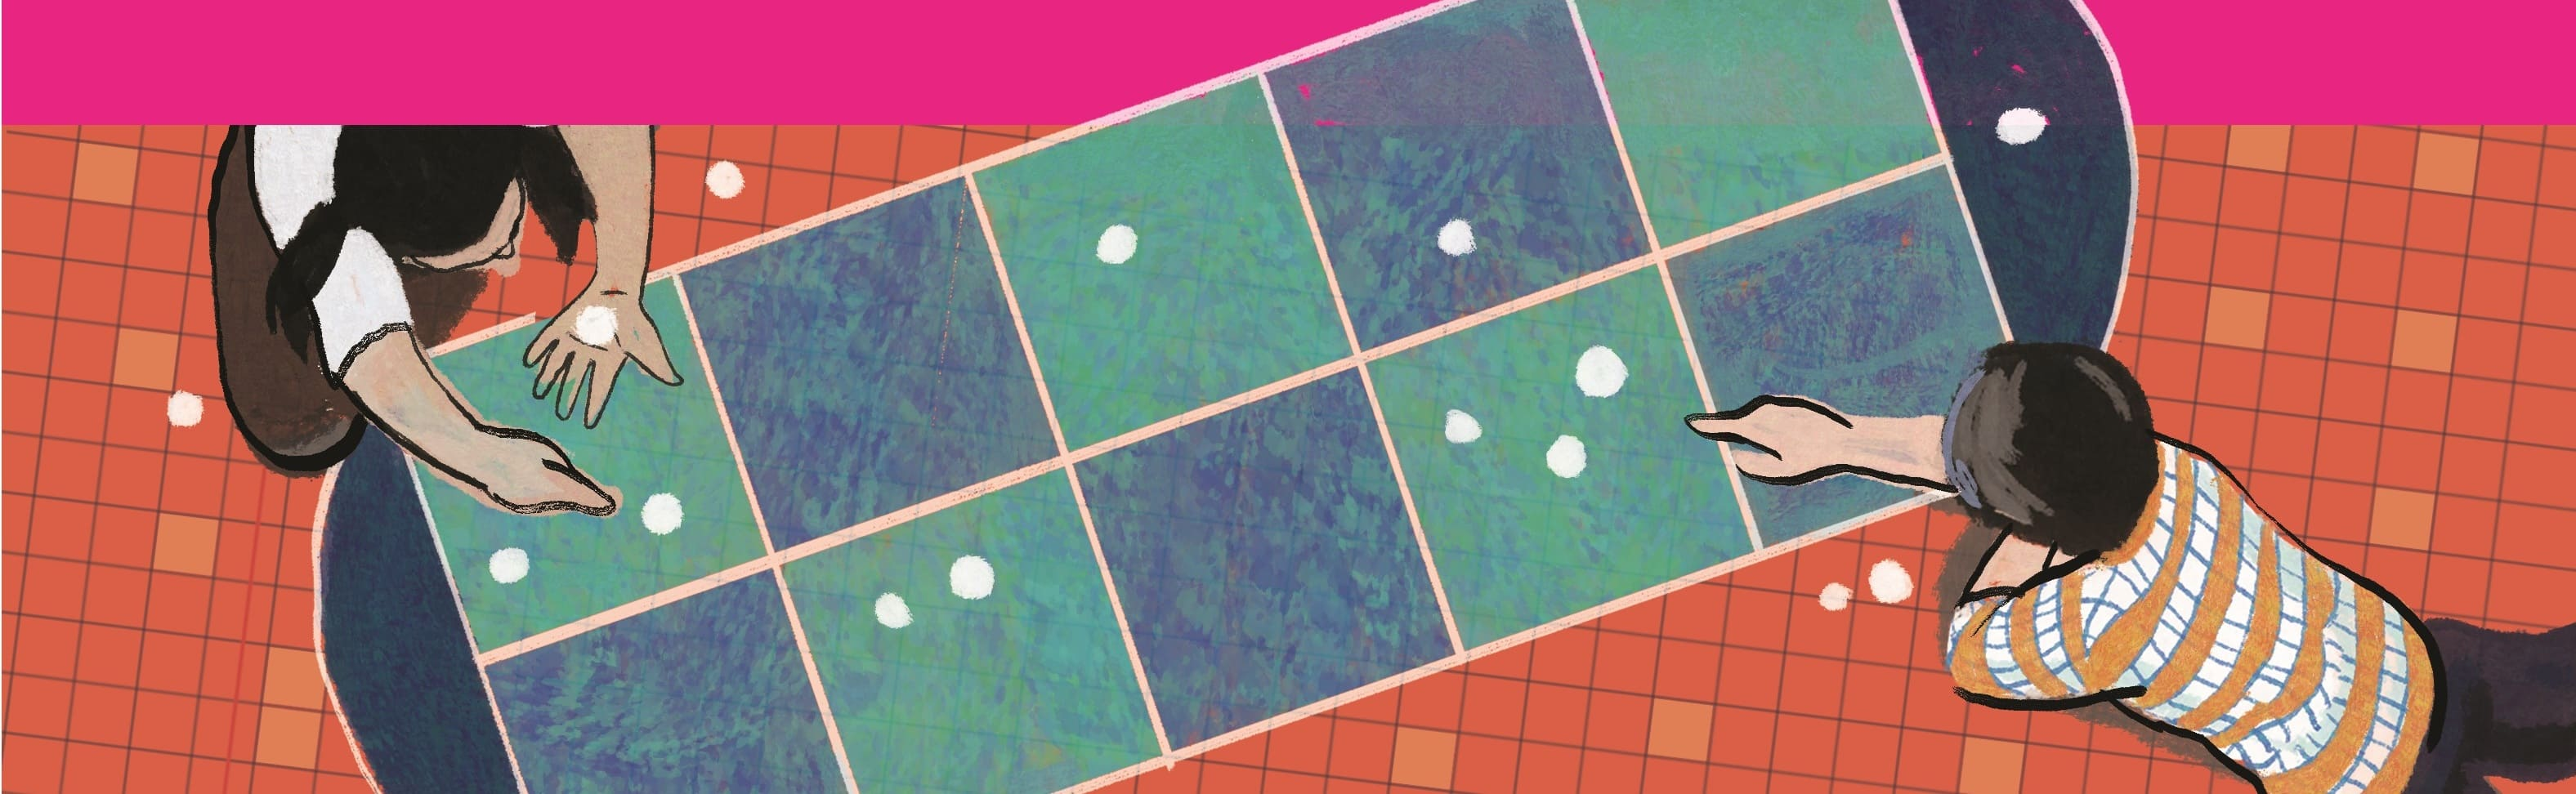
\includegraphics[width=19.3cm]{../bannertoancuabi}}}  
\AddToShipoutPicture*{\put(85,525){
\includegraphics[scale=1]{../tieude1.pdf}}} 
\centering
\endgroup

\vspace*{180pt}

\newpage
\begingroup
\thispagestyle{toancuabinone}
\blfootnote{$^1$\color{toancuabi}Ottawa, Canada.}
\AddToShipoutPicture*{\put(60,733){
\includegraphics[width=17.2cm]{../mathc.pdf}}}
%\AddToShipoutPicture*{\put(-2,733){
\includegraphics[width=17.2cm]{../mathl.pdf}}} 
\AddToShipoutPicture*{\put(172,675){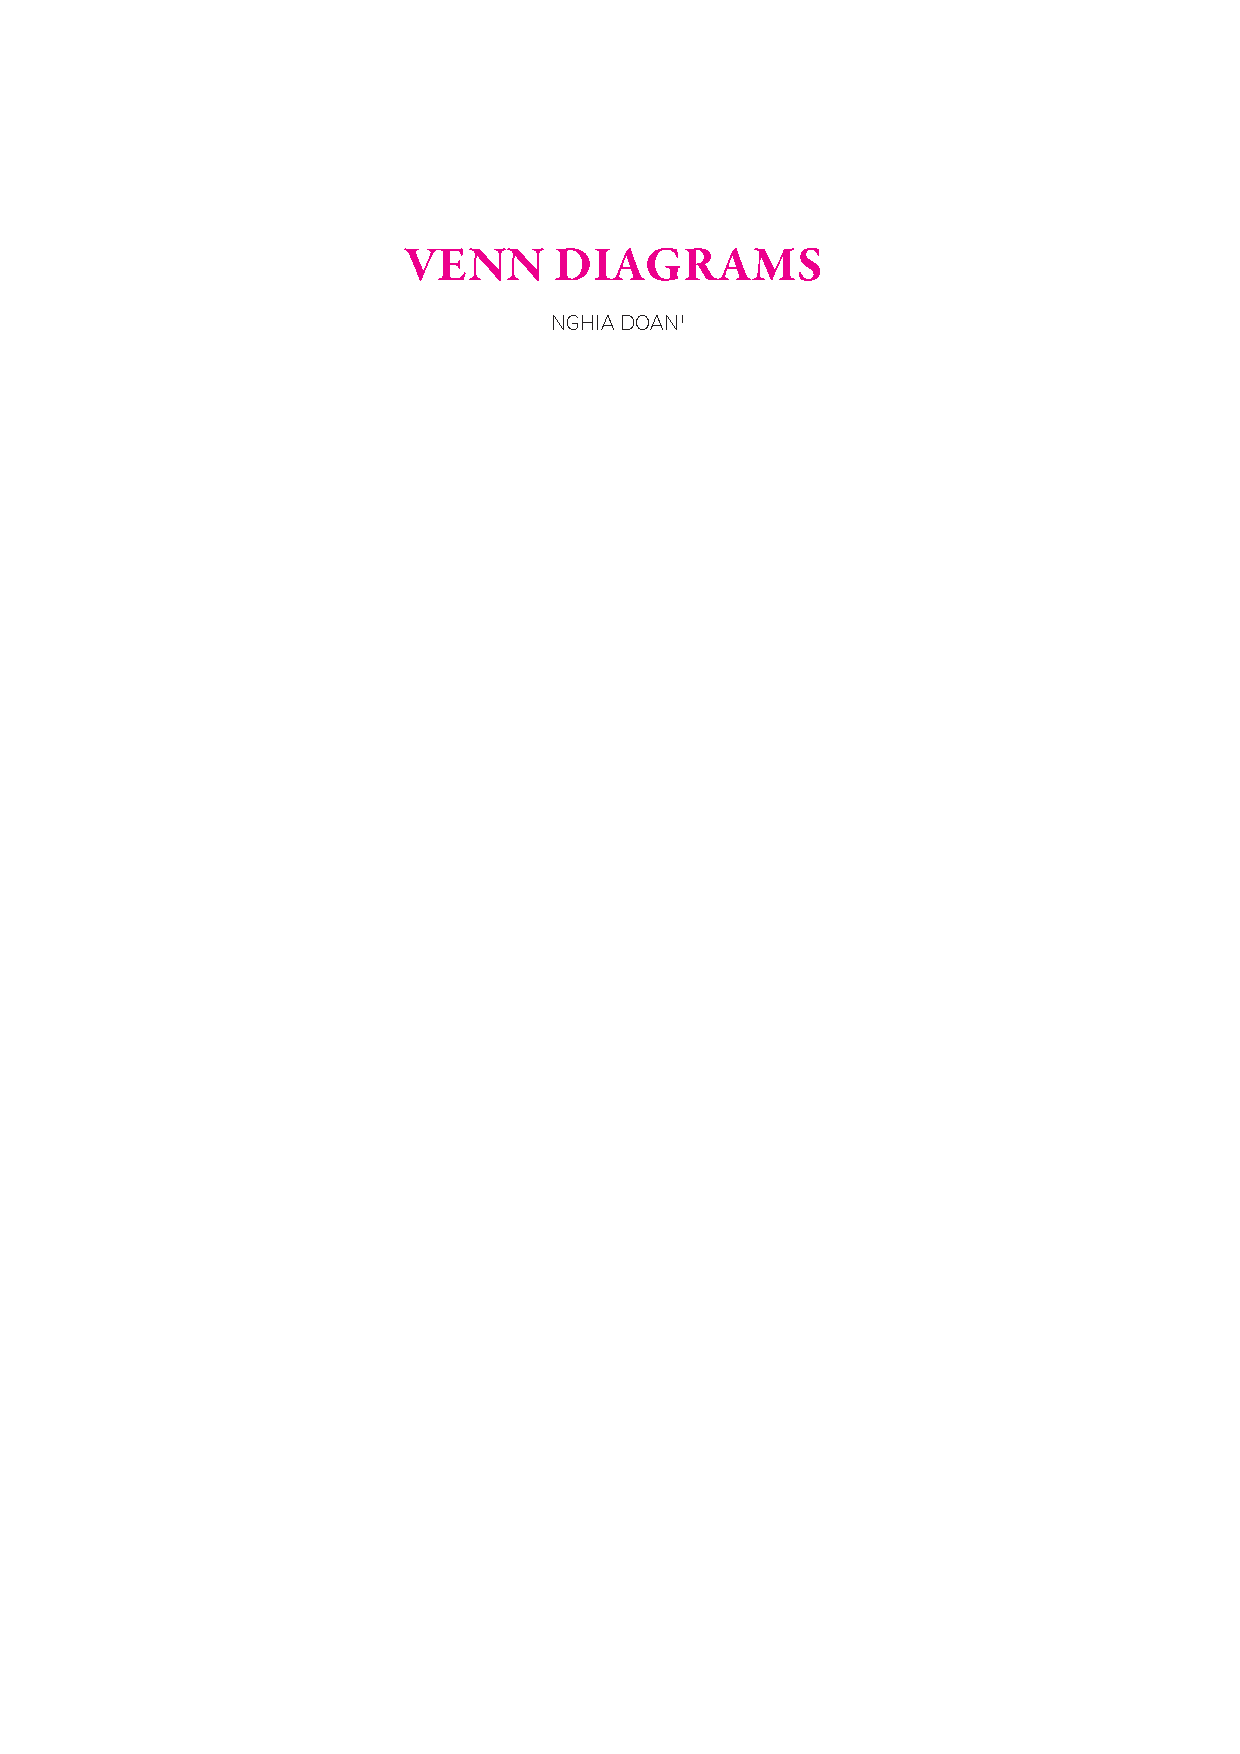
\includegraphics[scale=1]{../tieude4.pdf}}} 
\centering
\endgroup
\graphicspath{{../toancuabi/pic/}}
\vspace*{30pt}

\begin{multicols}{2}
	In this article, we explore the use of Venn diagrams through a few examples.
	\vskip 0.2cm
	\PIbox{\textbf{\color{toancuabi}Example} (Overlapping rugs)\textbf{\color{toancuabi}.}
		Three rugs have a combined area of $200$ $m^2.$ The rugs are overlapped as shown in the diagram below.
		The overlapped rugs together cover a floor area of $140$ $m^2.$ Furthermore the area covered by exactly any two rugs is $24$ $m^2$. 
		What is the are of floor is covered by all three rugs?}
	\vskip 0.1cm
	\begin{figure}[H]
		\vspace*{-5pt}
		\centering
		\captionsetup{labelformat= empty, justification=centering}
		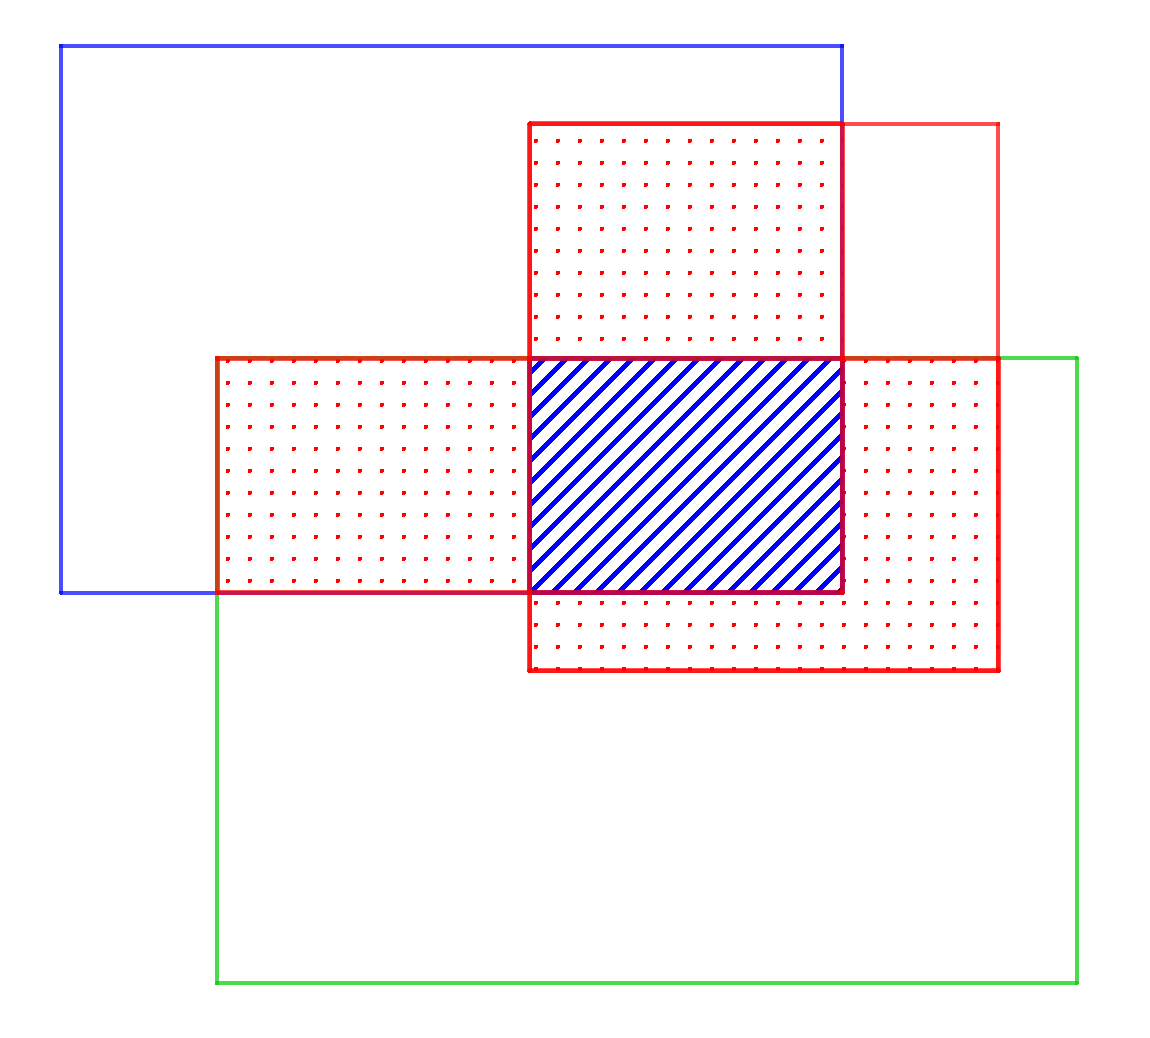
\includegraphics[width= 1\linewidth]{pi-2023-01-01.pdf}
		\vspace*{-10pt}
	\end{figure}
	\textit{Soluiton.}
	The total area of the three rugs, when not overlapping, is the sum of the areas of the three rectangles, which is $200$ $m^2.$
	The region show in the diagram above, formed by the overlapping rugs, has a total area of $140$ $m^2.$
	This means that $200-140=60$ $m^2$ is the total area of the three \textcolor{red}{red dotted parts},
	(because they are where the rugs overlapped once) plus twice \textcolor{blue}{the blue hatch part},
	(because it is where the rugs overlapped twice).
	\vskip 0.1cm
	In other words, if $r$ and $b$ are the areas of a red dotted and the blue hatch, respectively, then $3r + 2b = 60.$
	Furthermore, note that the area of a red dotted part plus the blue hatch part is $24$ $m^2,$ thus $r + b = 24.$
	Therefore $b = 3(r + b)- (3r+2b) = 3 \cdot 24 - 60 = \boxed{12}.$
	\vskip 0.1cm
	\PIbox{\textbf{\color{toancuabi}Exercise} (Overlapping circles)\textbf{\color{toancuabi}.}
		Three circles with radius $2, 3$ and $4$ are overlapping each other.
		The largest circle is partitioned into shaded region $A$ and unshaded regions $B$ and $C$.
		If the total area of the shaded region is $17\pi,$ what is the area of region $A$ in terms of $\pi$?}
	\vskip 0.1cm
	\begin{figure}[H]
		\vspace*{-5pt}
		\centering
		\captionsetup{labelformat= empty, justification=centering}
		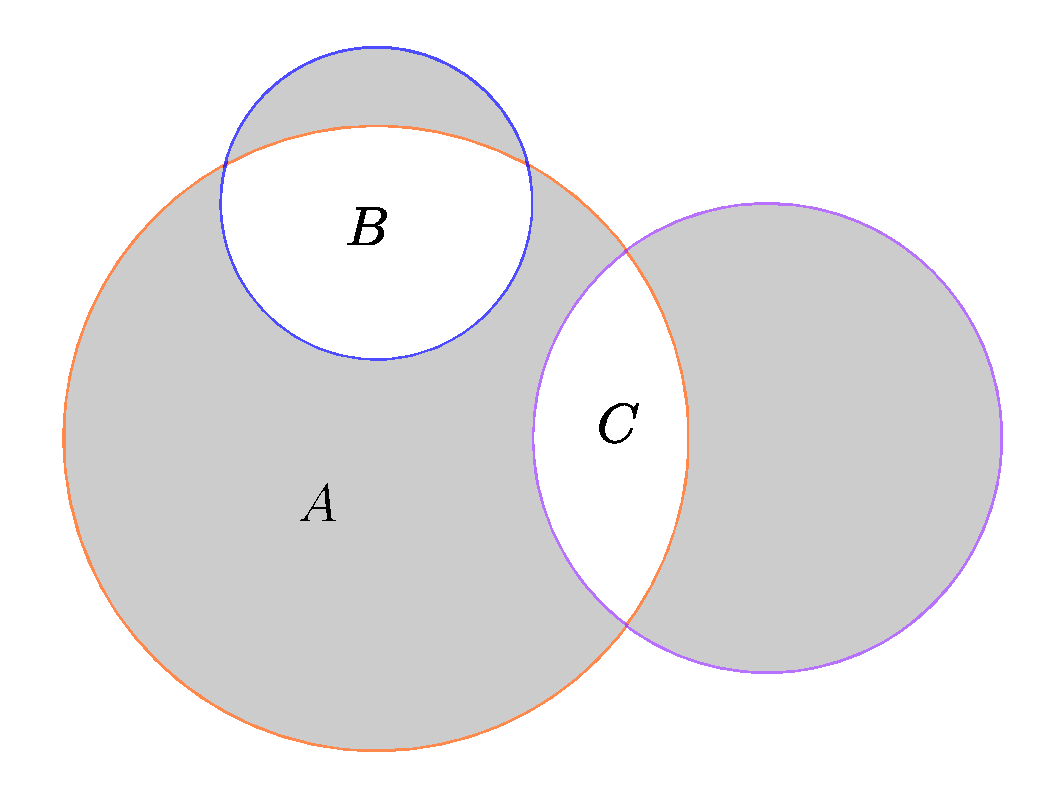
\includegraphics[width= 1\linewidth]{pi-2023-01-02.pdf}
		\vspace*{-10pt}
	\end{figure}
	\textit{Soluiton.}
	The total area of the circles is the area of the shaded region plus \textit{twice} the area of the unshaded regions:
	\begin{align*}
			4\pi + 9\pi + 16\pi = 17\pi + 2(B+C) \Rightarrow B+C = 6\pi \Rightarrow A = 16\pi - (B+C) = \boxed{10\pi}
	\end{align*}
	\PIbox{\textbf{\color{toancuabi}Example} (Alligators are ferocious and creepy crawlers)\textbf{\color{toancuabi}.}
	If all alligators are ferocious creatures and some creepy crawlers are alligators. It is easy to verify that:
	(i) all alligators are creepy crawlers; (ii) some ferocious creatures are creepy crawlers;
	and (iii) some alligators are not creepy creatures.
	\vskip 0.1cm
	Now, which statements below are true, false, or undecidable (you can't say it is true or false)?
	\vskip 0.1cm
	$S1.$ Some of creepy creatures are ferocious.
	\vskip 0.1cm
	$S2.$ Some ferocious creatures are creepy crawlers.
	\vskip 0.1cm
	$S3.$ Some alligators are not creepy creatures.
	\vskip 0.1cm
	$S4.$ Some ferocious crawlers are not alligators.
	\vskip 0.1cm
	$S5.$ Alligators are ferocious and creepy crawlers.}
	\vskip 0.2cm
	\textit{Solution.} To help the reasoning with visual cues, you can use Venn diagrams.
	\vskip 0.1cm
	First, we draw a \textcolor{red}{circle} depicting the set of alligators. In other words all alligators are in this circle.
	Since all alligators are ferocious creatures, thus the \textcolor{blue}{circle} containing all ferocious creatures must cover the circle of alligators .
	Now, some creepy crawlers are alligators, thus the \textcolor{green}{circle} containing all creepy crawlers must intersect and not contain the circle of alligators.
	Logically the circle of creepy crawlers then should intersect the circle of ferocious creatures and should not cover it.
	We got the diagram shown below.
	\begin{figure}[H]
		\vspace*{-5pt}
		\centering
		\captionsetup{labelformat= empty, justification=centering}
		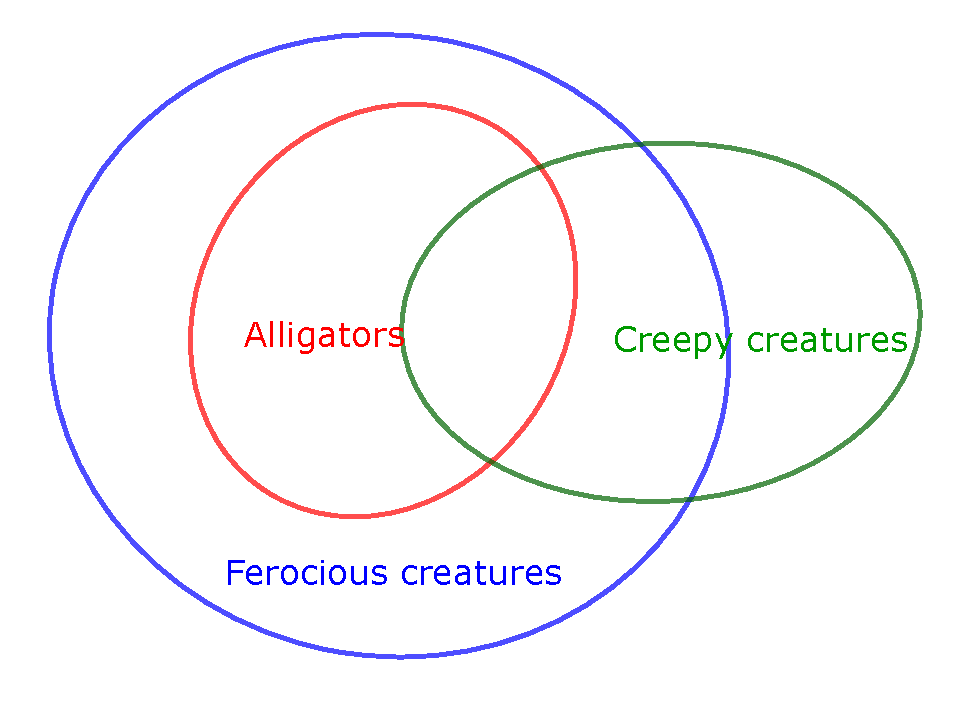
\includegraphics[width= 1\linewidth]{pi-2023-01-03.pdf}
		\vspace*{-10pt}
	\end{figure}	
	For $S1,$ those creepy crawlers are alligators, they must be in the intersection of the \textcolor{red}{circle} and \textcolor{green}{circle}.
	Since the \textcolor{red}{circle} resides within of the \textcolor{blue}{circle} the intersection must be part of the \textcolor{blue}{circle}.
	In other words those creepy crawlers are ferocious creatures. Thus the statement $B1$ is true.
	\vskip 0.1cm	
	It is also easy to verify that $S2$ is true.
	\vskip 0.1cm	
	Since we know that \textit{some creepy crawlers are alligators}, thus the \textcolor{green}{circle} intersect
	and may not contain the whole the \textcolor{red}{circle}, thus $S2$ is \textit{undecidable.}
	We don't know if some alligators are cute and not creepy.
	\vskip 0.1cm	
	The remaining two statements $S4$ and $S5$ are both \textit{undecidable}. Try to prove it yourself.
	\vskip 0.1cm
	\PIbox{\textbf{\color{toancuabi}Exercise} (Are boys good at math)\textbf{\color{toancuabi}.}
	Let assume that \textit{all boys in the math club are good at math.} 
	Which of the following statements must be true?
	\vskip 0.1cm
	$S1.$ No boy whose math is not good is a member of the math club.
	\vskip 0.1cm
	$S2.$ All boys whose math is good are members of the math club.
	\vskip 0.1cm
	$S3.$ All boys who are not members of the math club are not good at math.
	\vskip 0.1cm
	$S4.$ Every member of the math club whose math is good is a boy.
	\vskip 0.1cm
	$S5.$ There is one boy in the math club whose math is not good.
	\vskip 0.1cm
	Now decide that the following is true or false.
	\textit{A girl is good at math as a boy who is not member of the math club is not good as math as a boy who is member of the math club.}}
	\vskip 0.2cm
	\textit{Soluiton.} Draw three circles pairwise-intersecting each other, one labeled \textit{boys} (the girls are outside of this circle),
	the second other one labeled \textit{math} meaning whoever in this circle is good at math (the ones out side of it are not),
	and the third one labeled \textit{club} meaning whoever in this circle is member of the math club (the ones out side of it are not).
	None of the circle can contain another one. The club circle must cover the intersection of the boys and the math circle.
	A diagram is shown as below.
	\begin{figure}[H]
		\vspace*{-5pt}
		\centering
		\captionsetup{labelformat= empty, justification=centering}
		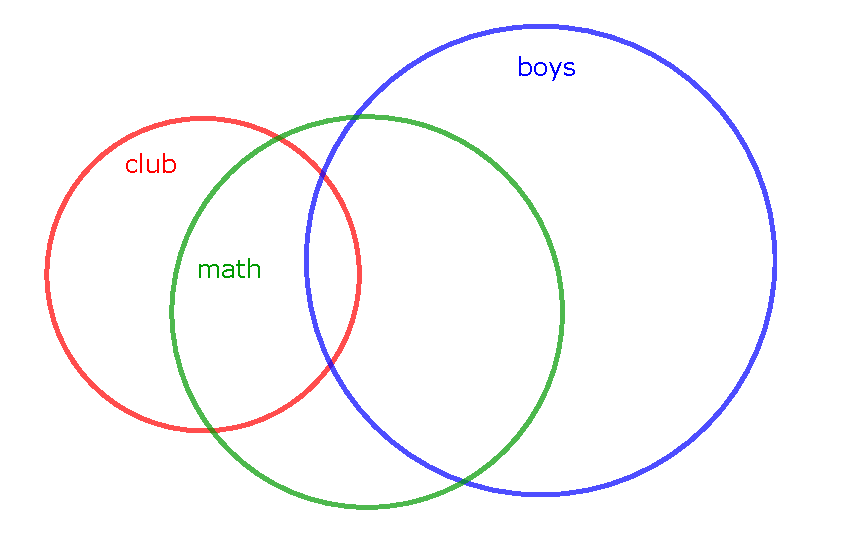
\includegraphics[width= 1\linewidth]{pi-2023-01-04.pdf}
		\vspace*{-10pt}
	\end{figure}	
	For $S2,S3, S4,$ and $S5,$ it is easy to find a counter example, thus none of them is true.
	$S1$ is true, otherwise if there were a boy whose math is not good and is a member of the math club,
	then because he is a member of the math club, his math has to be good. This contracdiction means the statement is true.
\end{multicols}